\section{Low-Dimensional Ordinary Least Squares}

  When you learn linear regression for the first time, you are really learning a very specific part of linear regression called ordinary least squares, which is the linear model that comes with a very specific loss function. Recall the \hyperref[fi-mse_loss]{MSE loss}.

  \begin{definition}[Ordinary Least Squares Regression]
    The \textbf{OLS linear regression} model is a linear regression model that tells us to minimize the MSE loss. 
  \end{definition}

  \begin{theorem}[Prediction Risk]
    The \textbf{prediction risk}\footnote{This is a bit different from how Wasserman defines it in his lectures, but I think this is better.} of $f$ is 
    \begin{equation}
      R(f) = \mathbb{E}_{x, y} [ (y - f(x))^2 ] = \mathbb{E}_{x, y} [ (y - \beta^T x)^2 ] 
    \end{equation}
    and the empricial risk is 
    \begin{equation}
      \hat{R}(f) = \frac{1}{n} \sum_{i=1}^n (y^{(i)} - f(x^{(i)}))^2 = \frac{1}{n} \| Y - X\beta\|^2
    \end{equation}
    where $X \in \mathbb{R}^{n \times d}$ is the data matrix where the $i$th row is sample $x^{(i)}$, and $Y \in \mathbb{R}^{d}$ is the vector of sample predictors. 
  \end{theorem}

  This is a bit weird, since we are just \textit{given} a loss function rather than having derived one from our model. There are two paths that we can take to derive this loss function. 
  \begin{enumerate}
    \item The first is to have the extra convenient assumption that the errors $\epsilon$ are Gaussian. This is not too unrealistic since combinations of many random noise gives us a Gaussian by the CLT. As often done in machine learning, by computing the likelihood, we can take its negative logarithm to get our loss. 
    \item The second does \textit{not} assume a distribution on $\epsilon$ and rather uses the Gauss-Markov theorem to directly say that the MSE loss minimizes variance among unbiased estimators. This is in a sense more fundamental. 
  \end{enumerate}
  Sometimes, the Gaussian error is given as an assumption, and sometimes it is not. We will go through all these points by first talking about the nice bias-variance decomposition of the MSE loss. Then, we will use the Gauss-Markov theorem justify the MSE loss and introduce the least-squares solution. Finally, we will look at the likelihood approach using Gaussian residuals. 

\subsection{Least Squares Solution} 

  Using simple calculus, we can simply find the point $\beta$ where the derivative of the loss is $0$. 
 
  \begin{theorem}[Least Squares Solution For Linear Regression]
    The solution that minimizes the MSE is 
    \begin{equation}
      \beta = (X^T X)^{-1} X^T Y 
    \end{equation}
  \end{theorem}
  \begin{proof}
    We simply minimize 
    \begin{align}
      L(\beta) = \|Y - X \beta\|^2 = \langle Y - X \beta, Y - X \beta \rangle \\ 
      & = (Y - X \beta)^T (Y - X \beta) \\ 
      & = Y^T Y - \beta^T X^T Y - Y^T X \beta + \beta^T X^T X \beta \\
      & = Y^T Y - 2 Y^T X \beta + \beta^T X^T X \beta 
    \end{align}
    where we omit the constant term because it doesn't affect the argmin. Taking the derivative\footnote{Remember the following matrix derivative rules when differentiating with respect to vector $x$. $\frac{\partial}{\partial x} x^T A = A$, $\frac{\partial}{\partial x} x^T A x = 2 Ax$. } and setting it equal to $0$ gives 
    \begin{align}
    \frac{\partial L}{\partial \beta} = - 2 X^T Y + 2 X^T X \beta = 0  
    & \implies X^T X \beta = X^T Y \\ 
    & \implies \hat{\beta} = (X^T X)^{-1} X^T Y
    \end{align}
  \end{proof} 

  \begin{example}[Simulation]
    Let's do this for a simple dataset of $200$ points across $10$ covariates with some noise $\epsilon \sim N(0, 0.01)$. 
    \begin{lstlisting}
      >>> import numpy as np 
      >>> n, d = 200, 10
      >>> beta_true = np.array([1, 2, 3, 1, -2, -3, 1, -2, 3, -1])
      >>> X = np.random.randn(n, d)
      >>> Y = X.dot(beta_true) + 0.1 * np.random.randn(n)
      >>> beta_hat = np.linalg.inv(X.T @ X) @ X.T @ Y 
      >>> print(beta_hat)
      [ 1.00981636  1.99629568  2.99167398  0.98981948 -1.99678893 -2.99819217
        0.99060477 -1.99468555  2.99490104 -0.99246088]
    \end{lstlisting} 
    We can clearly see that we have good approximates on this. 
  \end{example}

  \begin{corollary}[Variance of MSE Minimizer]
    The variance of the MSE minimizer with respect to $Y$ is 
    \begin{equation}
      \Var(\hat{\beta}) = \hat{\sigma}^2 (X^T X)^{-1} \in \mathbb{R}^{d \times d}
    \end{equation}
  \end{corollary}
  \begin{proof}
    We can calculate the variance of $\beta$ by using the fact that $\Var[A X] = A \Var[X] A^T$, is
    \begin{equation}
      \Var(\hat{\beta}) = (X^{T} X)^{-1} X^{T} \;\sigma^2 I \; X  (X^{T} X)^{-1} = \sigma^2 (X^{T} X)^{-1} (X^{T} X)  (X^{T} X)^{-1} = \sigma^2  (X^{T} X)^{-1}
    \end{equation}
    But we don't know the true $\sigma^2$, so we estimate it with $\hat{\sigma}^2$ by taking the variance of the residuals. Therefore, we have 
    \begin{align}
      \beta & = (X^T X)^{-1} X^T Y \in \mathbb{R}^d \\
      \Var(\hat{\beta}) & = \hat{\sigma}^2 (X^T X)^{-1} \in \mathbb{R}^{d \times d}
    \end{align}
  \end{proof}

  \begin{example}[Simulation]
    Let's empirically demonstrate the previous theorem by taking a dataset of fixed $X$, and then generating the $Y$ $10000$ times. For each $Y$ we train $\hat{\beta}$, and take the sample covariance. For conciseness, we only print the top-left $3 \times 3$ block matrix. 

    \begin{lstlisting}
      >>> import numpy as np 
      >>> n, d = 200, 10
      >>> beta_true = np.array([1, 2, 3, 1, -2, -3, 1, -2, 3, -1])
      >>> X = np.random.randn(n, d)
      >>> def run(): 
      ...   Y = X.dot(beta_true) + 0.1 * np.random.randn(n)
      ...   beta_hat = np.linalg.inv(X.T @ X) @ X.T @ Y 
      ...   return beta_hat
      ... 
      >>> 
      >>> true_cov = 0.1 * np.linalg.inv(X.T.dot(X)) 
      >>> print(true_cov[:3, :3]) # True covariance according to our theorem
      [[ 5.51430990e-04  1.04398204e-05 -4.60641482e-06]
       [ 1.04398204e-05  5.82171568e-04 -1.70354446e-05]
       [-4.60641482e-06 -1.70354446e-05  4.38241743e-04]]
      >>> betas = np.stack([run() for _ in range(10000)], axis=0)
      >>> print(np.cov(betas.T)[:3, :3]) # estimated sample covariance
      [[ 5.55882814e-05  5.47990882e-07 -4.53151038e-07]
       [ 5.47990882e-07  5.89809163e-05 -2.02919464e-06]
       [-4.53151038e-07 -2.02919464e-06  4.37200525e-05]]
      >>> 
    \end{lstlisting}
  \end{example}

  Note that we have assumed that $X^T X$ was invertible in order for such a solution to be unique, i.e. $X$ must be full rank. This process breaks down when it isn't invertible, e.g. if there are repetitions in the features (one feature is a linear combination of the others and hence not full column rank). We will talk more about this soon. 

  \begin{definition}[Hat Matrix]
    The \textbf{hat matrix} is defined 
    \begin{equation}
      H = X (X^T X)^{-1} X^T \in \mathbb{R}^{n \times n}
    \end{equation}
    It is the projection of the observed $y^{(i)}$'s to the least squared predictions.\footnote{It projects to the column space of $X$.} 
    \begin{equation}
      \hat{Y} = H Y
    \end{equation}
  \end{definition}

  We can also see that the residuals $\hat{\epsilon}_i = y_i - \hat{y}_i$ has the property that 
  \begin{equation}
    \hat{\epsilon} = y - \hat{y} = (I_n - H) y 
  \end{equation}

  Note that this parallels the orthogonal projection of conditional expectation to the true function onto the subspace of $X$ measurable functions. Except that we are not doing this in function space, but rather the sample space $\mathbb{R}^n$. 

  \begin{example}[Copying Data]
    What happens if you copy your data in OLS? In this case, our MLE estimate becomes 
    \begin{align*}
        \left(\begin{pmatrix}X \\ X \end{pmatrix}^T \begin{pmatrix} X \\ X \end{pmatrix} \right )^{-1} & \begin{pmatrix} X \\ X  \end{pmatrix}^T \begin{pmatrix} Y \\ Y  \end{pmatrix}  =\\
    & = (X^T X + X^T X)^{-1} (X^T Y + X^T Y ) = (2 X^T X)^{-1} 2 X^T Y = \hat{\beta}
    \end{align*}
    and our estimate is unaffected. However, the variance shrinks by a factor of $2$ to 
    \begin{equation}
      \frac{\sigma^2}{2} (X^T X)^{-1}
    \end{equation}
    A consequence of that is that confidence intervals will shrink with a factor of $1/\sqrt{2}$. The reason is that we have calculated as if we still had iid data, which is untrue. The pair of doubled values are obviously dependent and have a correlation of $1$. 
  \end{example}

\subsection{Gauss Markov Theorem}

  Now recall from our \hyperref[fi-bias_variance_mse]{frequentist inference notes} that with the MSE loss, we have the bias-variance-noise decomposition as 
  \begin{align}
    \mathbb{E}_{\mathcal{D}} \mathbb{E}_{x, y} \big[ (y - \hat{f}_{\mathcal{D}}(x))^2 \big] 
    & = \mathbb{E}_{x} \big[ \underbrace{ \big( \mathbb{E}[y \mid x] - \mathbb{E}_{\mathcal{D}} [\hat{f}_\mathcal{D} (x)] \big)^2}_{\text{(expected bias)}^2} \big] + \underbrace{ \mathbb{E}_\mathcal{D} \big[ \mathbb{E}_{x} \big[ \big( \mathbb{E}_\mathcal{D} [\hat{f}_\mathcal{D} (x)] - \hat{f}_\mathcal{D} (x) \big)^2 \big] \big]}_{\text{expected variance}} \\ 
    & \;\;\;\;\;\;\;\;\;\;\;\;\;\;\;\;\;\;\;\;\;\;\;\;\; + \underbrace{\mathbb{E}_{x, y} [(y - \mathbb{E}[y \mid x])^2]}_{\text{noise}}
  \end{align}

  \begin{theorem}[Gauss-Markov Theorem]
    Given a dataset with 
    \begin{enumerate}
      \item mean zero residuals $\mathbb{E}[\epsilon_i] = 0$, i.e. $\mathbb{E}[\mathbf{Y} \mid \mathbf{X}] = \mathbf{X} \boldsymbol{\beta}$. 
      \item homoscedacity $\mathrm{Var}[\epsilon_i] = \sigma^2 < \infty$ for all $i$, 
      \item uncorrelated residuals $\mathrm{Cov}(\epsilon_i, \epsilon_j) = 0$ for all $i \neq j$. This and the previous assumption can be combined into $\mathrm{Cov}[\mathbf{Y} \mid \mathbf{X}] = \sigma^2 \mathbf{I}_n$. 
    \end{enumerate}
    We were concerned with estimating the parameters $\beta_1, \ldots, \beta_d$. Now let's generalize this and consider the problem of estimating, for some known constants $c_1, \ldots, c_{d+1}$, the point estimator 
    \begin{equation}
      \theta = c_1 \beta_1 + c_2 \beta_2 + \ldots + c_d \beta_d + c_{d+1}
    \end{equation}
    Then the estimator 
    \begin{equation}
      \hat{\theta} = c_1 \hat{\beta}_1 + c_2 \hat{\beta}_2 + \ldots + c_d \hat{\beta}_d + c_{d+1}
    \end{equation}
    where $\hat{\beta_i}$ is clearly an unbiased estimator of $\theta$ and it is a linear estimator of $\theta$, i.e. 
    \begin{equation}
      \hat{\theta} = \sum_{i=1}^n b_i y_i
    \end{equation}
    for some known (given $\mathbf{X}$) constants $b_i$. Then, the Gauss-Markov theorem states that the estimator $\hat{\theta}$ has the smallest (best) variance among \textit{all} linear unbiased estimators of $\theta$, i.e. $\hat{\theta}$ is BLUE. 
  \end{theorem}

\subsection{Likelihood Estimation}

  Now we add the \textit{additional} assumption that the residuals are distributed according to a Gaussian. This gives us a parameteric closed-form of our likelihood, which we can then maximize with respect to $\beta$. The likelihood is simple to compute. 

  \begin{lemma}[Likelihood]
    Given a dataset $\mathcal{D} = \{(x^{(i)}, y^{(i)})\}_{i=1}^N$, our likelihood is 
    \[L(\beta ; \mathcal{D}) = \prod_{i=1}^N p(y^{(i)} \mid x^{(i)}; \beta) = \prod_{i=1}^N \frac{1}{\sqrt{2 \pi \sigma^2}} \exp \bigg( -\frac{(y^{(i)} - \beta^T x^{(i)})^2}{2 \sigma^2} \bigg)\]
  \end{lemma} 

  \begin{theorem}[Negative Log-Likelihood is MSE Loss]
    We can take its negative log, remove additive constants, and scale accordingly to get 
    \begin{align}
      \ell (\beta) & = -\frac{N}{2} \ln{\sigma^2} - \frac{N}{2} \ln(2 \pi) + \frac{1}{2 \sigma^2} \sum_{i=1}^N \big(y^{(i)} - \beta^T x^{(i)} \big)^2 \\
      & =\frac{1}{2} \sum_{i=1}^N \big(y^{(i)} - \beta^T x^{(i)} \big)^2 
    \end{align}
    which then corresponds to minimizing the sum of squares error function. 
  \end{theorem}

  So assuming Gaussian residuals also gives us back the MSE as a natural loss function. This is usually the way that beginners tend to use the loss function, but this is not as general as the Gauss-Markov theorem, which is \textit{distribution-free}. As soon as we have the same loss, it should be clear that the MLE is the same as the least-squares optimizer. 

  \begin{corollary}[MLE is the Same as Least-Squares Estimator]
    The MLE is 
    \begin{equation}
      \hat{\beta} = (X^T X)^{-1} X^T Y
    \end{equation}
    which is the same as the least squares estimator. We have an additional nusiance parameter $\sigma^2$, however, and the MLE is 
    \begin{equation}
      \hat{\sigma}^2 = \frac{1}{n} \sum_{i=1}^n \big( y^{(i)} - \hat{\beta}^T x^{(i)} \big)^2
    \end{equation}
    where $\hat{\beta}$ is already solved. 
  \end{corollary}
  \begin{proof}
    This is not needed, but let's go through the computations anyways. Taking the gradient of this log likelihood w.r.t. $\beta$ gives 
    \begin{equation}
      \nabla_\beta \ell (\beta) = \sum_{i=1}^n ( y^{(i)} - \beta^T x^{(i)}) x^{(i)}
    \end{equation}
    Note that since we can solve this in closed form, by setting the gradient to $0$, we have 
    \begin{equation}
      0 = \sum_{i=1}^n y^{(i)} x^{(i) T} - \beta^T \bigg( \sum_{i=1}^n x^{(i)} x^{(i) T} \bigg)
    \end{equation}

    which is equivalent to solving the least squares equation 
    \begin{equation}
      \beta = ( X^T X)^{-1} X^T Y
    \end{equation}
  \end{proof}

  Now note that matrix inversion and multiplication are of cubic time complexity. This may be an actual problem when either $n$ or $d$ is large. Therefore, we can simply numerically optimize it with stochastic gradient descent. Over a minibatch $M \subset \mathcal{D}$, we have 
  \begin{align}
    \beta & = \beta - \eta \nabla_\beta \ell (\beta) \\
    & = \beta - \eta \sum_{(x, y) \in M} (\beta^T x - y) x
  \end{align}
  This is guaranteed to converge since $\ell(\beta)$, as the sum of convex functions, is also convex.  

  \begin{example}[SGD From Scratch]
    Let's see this in action. 

    \begin{lstlisting}
      >>> import numpy as np 
      >>> n, d = 200, 5
      >>> beta_true = np.array([1, 2, 3, 1, -2])
      >>> X = np.random.randn(n, d)
      >>> Y = X.dot(beta_true) + 0.1 * np.random.randn(n)
      >>> # Gradient descent 
      >>> lr = 1e-2
      >>> beta_hat = np.random.randn(5)
      >>> for _ in range(1000): 
      ...   grad = (1/200) * np.sum((Y - X.dot(beta_hat)).reshape(-1, 1) * X, axis=0)
      ...   beta_hat += lr * grad  
      ... 
      >>> 
      >>> print(beta_hat)
      [ 1.01353957  1.99694533  2.99698439  1.00279151 -2.00176132]
    \end{lstlisting}

    Note that this is sensitive to numerical errors if we set the learning rate to be too high. On the other hand, it may not converge fast enough if we set the learning rate too low. The following are after 1000 steps of convergence. 

    \begin{lstlisting}
      lr: 10.0
      [nan nan nan nan nan]
      lr: 1.0
      [ 0.99783623  2.00872921  3.00480298  1.00303178 -2.00464259]
      lr: 0.1
      [ 0.99783623  2.00872921  3.00480298  1.00303178 -2.00464259]
      lr: 0.01
      [ 0.99680738  2.00773822  3.00377349  1.00355067 -2.00464062]
      lr: 0.001
      [ 0.38075539  0.56665193  1.13758925  0.80863722 -1.51169666]
      lr: 0.0001
      [-0.12150123 -0.11091773  0.47147945  0.14935135 -0.28254488]
    \end{lstlisting}
  \end{example}

  \begin{code}[OLS Linear Regression in scikit-learn]
    Here is a minimal working example of performing linear regression with scikit-learn. Note that the input data must be of shape $(n, d)$. 

    \noindent\begin{minipage}{.6\textwidth}
    \begin{lstlisting}[]{Code}
      import numpy as np 
      from sklearn.linear_model import LinearRegression 
      X = np.array([[1, 1], [1, 2], [2, 2], [2, 3]]) 
      y = np.dot(X, np.array([1, 2])) + 3 
      model = LinearRegression()  
      model.fit(X, y) 
      print(X) 
      print(y)
      print(model.score(X, y))  
      print(model.intercept_)
      print(model.coef_) 
      print(model.predict(np.array([[3, 5]])))
    \end{lstlisting}
    \end{minipage}
    \hfill
    \begin{minipage}{.39\textwidth}
    \begin{lstlisting}[]{Output}
      [[1 1]
       [1 2]
       [2 2]
       [2 3]]
      [ 6  8  9 11]
      1.0
      3.0000000000000018
      [1. 2.]
      [16.]
      .
      .
      .
    \end{lstlisting}
    \end{minipage}
  \end{code}

\subsection{Coefficient of Determination} 

  We now suggest a more interpretable metric for a linear regression model. Say that we did not have any of the $X$ data and were told to try and predict the $Y$'s according to the MSE loss. The best we can do is simply compute their mean, and our regression function would always be 
  \begin{equation}
    f(x) = \bar{Y} \approx \mathbb{E}_y[y]
  \end{equation}
  Rather than thinking of this as a sum of squared errors, we can think of this in term of variance. If we had our naive model above, then our sums of squares errors is equal to the sample variance. 
  \begin{equation}
    \frac{1}{n} \sum_{i=1}^n \left( y^{(i)} - f(x^{(i)}) \right)^2 = \frac{1}{n} \sum_{i=1}^n \left( y^{(i)} - \bar{y} \right)^2  
    \approx \Var_y [y]
  \end{equation}
  This is not a very good approximation, and this is shown by a large amount of variance that is not captured. 

  \begin{definition}[Total Sum of Squares]
    The \textbf{total sum of squares} is defined 
    \begin{equation}
      TSS = \frac{1}{n} \sum_{i=1}^n \left( y^{(i)} - \bar{y} \right)^2
    \end{equation}
  \end{definition} 

  What we want to do is \textit{reduce} this variance by having better estimates of the mean $\bar{y}$. Now if we are given the $x$, perhaps using the $x$'s to model a better mean of $y$ through $f$ might help, and doing this will lead to a hopefully lower variance, i.e. the \textit{residual sum of squares}. 

  \begin{definition}[Residual Sum of Squares]
    The \textbf{residual sum of squares} is defined 
    \begin{equation}
      RSS = \frac{1}{n} \sum_{i=1}^n \left( y^{(i)} - f(x^{(i)}) \right)^2 
    \end{equation}
  \end{definition} 

  If we have a TSS of $2$ and a RSS of $1$, then we have decreased our variance by 50\%. We can formalize this into the following. 

  \begin{definition}[Coefficient of Determination]
    The \textbf{coefficient of determination} is the proportion of the variation in the dependent variable that is predictable from the independent variables It is defined 
    \begin{equation}
      R^2 = 1 - \frac{RSS}{TSS}
    \end{equation}
    and $R^2$ value of $1$ represents the best model. 
  \end{definition}

  However, a drawback of $R^2$ is that it always increases if we add predictors to the regression model, leading to a possible overfitting. 

  \begin{example}[RSS and $R^2$ Values as we Account for More Covariates]
    \begin{lstlisting}
      import numpy as np
      import matplotlib.pyplot as plt

      n, d = 200, 10
      beta_true = np.array([1, 2, 3, 1, -2, 1, 2, 3, 1, -2])
      X = np.random.randn(n, d)
      Y = X.dot(beta_true) + 0.1 * np.random.randn(n) 

      RSSs = []
      R2s = []
      TSS = np.var(Y)
      RSSs.append(TSS)
      R2s.append(0)

      for k in range(1, 11): 
          X_trunc = X[:,:k]
          beta_hat = np.linalg.inv(X_trunc.T @ X_trunc) @ X_trunc.T @ Y 
          RSS = np.var(Y - X_trunc.dot(beta_hat)) 
          R2 = 1 - RSS/TSS  
          RSSs.append(RSS) 
          R2s.append(R2)

      fig, (ax1, ax2) = plt.subplots(1, 2, figsize=(12, 5))

      ax1.plot(range(11), RSSs, 'r-', marker='o')
      ax1.set_title('Residual Sum of Squares (RSS)')
      ax1.set_xlabel('Number of Features')
      ax1.set_ylabel('RSS')
      ax1.grid(True, alpha=0.3)

      ax2.plot(range(11), R2s, 'b-', marker='o')
      ax2.set_title('R-squared')
      ax2.set_xlabel('Number of Features')
      ax2.set_ylabel('R2')
      ax2.grid(True, alpha=0.3)

      plt.tight_layout()
      plt.show() 
    \end{lstlisting} 
    This gives the following plot. You can indeed see that the RSS is monotonically decreasing and the $R^2$ is monotonically increasing as we add more covariates. 

    \begin{figure}[H]
      \centering 
      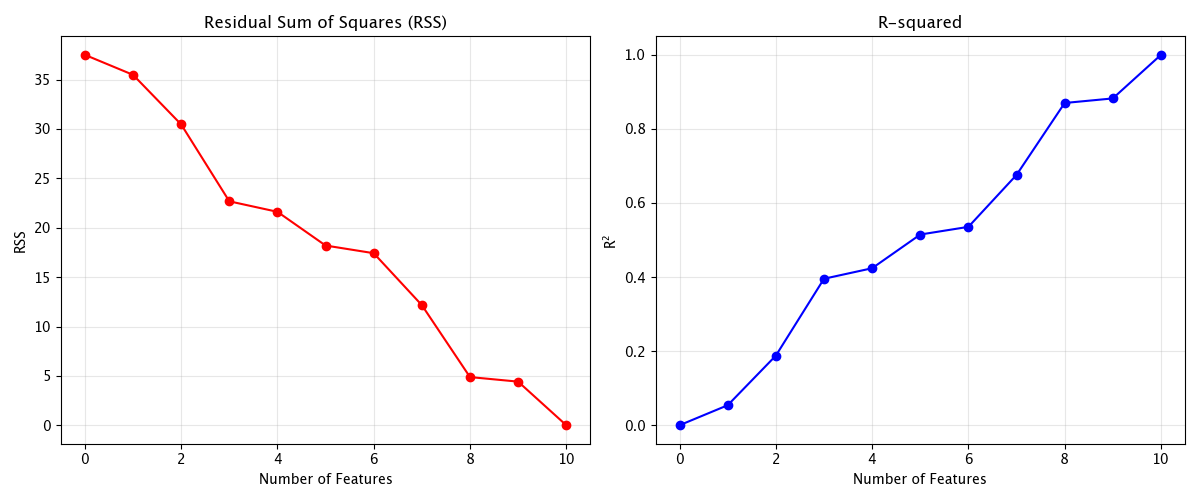
\includegraphics[scale=0.4]{img/rss_r2.png}
      \caption{Note that the steps at which the RSS decrease the most are precisely the covariates where its true values are largest. The first covariate (true value of $1$) doesn't decrease the RSS too much, but as we add the second (true value $2$) and third ($3$), the RSS decreases much sharply. } 
    \end{figure}
  \end{example}

  There are cases when the $RSS > TSS$, leading to a negative $R^2$ value. This essentially means that the model is doing worse than just taking the mean. 

\subsection{Simple Linear Regression}

  The simple linear regression is the special case of the linear regression with only one covariate.\footnote{I've included a separate section on this since this was especially important for quant interviews.} Interviewers like this model for its aesthetically pleasing theoretical properties. We will just list a bunch of them. 


  \begin{definition}[Simple Linear Regression]
    We will use the following notation. 
    \begin{equation}
      y = \alpha + x \beta
    \end{equation}
  \end{definition}

  \begin{theorem}[Best Fit]
    The least-squares best fit is 
    \begin{align}
      \hat{\beta} & = \frac{\sum_i (x_i - \bar{x}) (y_i - \bar{y})}{\sum_i (x_i - \bar{x})^2} = \frac{\mathrm{cov}(x, y)}{\mathrm{var}(x)} = \rho_{xy} \frac{s_y}{s_x}
    \end{align}
    where $\rho_{xy}$ is the correlation between $x$ and $y$, and the variance and covariance represent the sample variance and covariance (indicated in lower case letters). Therefore, the correlation coefficient $\rho_{xy}$ is precisely equal to the slope of the best fit line when $x$ and $y$ have been standardized first, i.e. $s_x = s_y = 1$. 
  \end{theorem}
  \begin{proof}
    For $n$ pairs of $(x_i, y_i)$, 
    \begin{equation}
      y_i = \alpha + \beta x_i + \epsilon_i
    \end{equation}

    To minimize the sum of squared errors 
    \begin{equation}
      \sum_{i} \epsilon_i^2 = \sum_{i} (y_i - \alpha - \beta x_i)^2
    \end{equation}

    Taking the partial derivatives w.r.t. $\alpha$ and $\beta$ and setting them equal to $0$ gives 
    \begin{align}
      &\sum_i (y_i - \hat{\alpha} - \hat{\beta} x_i) = 0 \\
      &\sum_i (y_i - \hat{\alpha} - \hat{\beta} x_i) x_i = 0
    \end{align}

    From just the first equation, we can write 
    \begin{equation}
      n \bar{y} = n \hat{\alpha} + n \hat{\beta} \bar{x} \implies y = \hat{\alpha} + \hat{\beta} \bar{x} \implies \hat{\alpha}  = \bar{y} - \hat{\beta} \bar{x} 
    \end{equation}

    The second equation gives 
    \begin{equation}
      \sum_{i} x_i y_i = \hat{\alpha} n \bar{x} + \hat{\beta} \sum_{i} x_i^2
    \end{equation}

    and substituting what we derived gives 
    \begin{align}
      \sum_{i} x_i y_i & = (\bar{y} - \hat{\beta} \bar{x}) n \bar{x} + \hat{\beta} \sum_i x_i^2 \\
      & = n \bar{x} \bar{y} + \hat{\beta} \bigg( \Big(\sum_i x_i^2 \Big) - n \bar{x}^2 \bigg)
    \end{align}

    and so we have 
    \begin{equation}
      \hat{\beta} = \frac{ \big( \sum_i x_i y_i \big) - n \bar{x}\bar{y}}{\big( \sum x_i^2 \big) - n \bar{x}^2} = \frac{ \sum_i x_i y_i - \bar{x} y_i}{\sum x_i^2 - \bar{x} x_i} = \frac{ \sum_i (x_i - \bar{x}) y_i}{\sum_i (x_i - \bar{x}) x_i}
    \end{equation}

    Now we can use the identity
    \begin{align}
      \sum_{i} (x_i - \bar{x}) (y_i - \bar{y}) & = \sum_i y_i (x_i - \bar{x}) = \sum_i x_i (y_i - \bar{y}) 
    \end{align}

    to substitute both the numerator and denominator of the equation to 
    \begin{align}
      \hat{\beta} & = \frac{\sum_i (x_i - \bar{x}) (y_i - \bar{y})}{\sum_i (x_i - \bar{x})^2} = \frac{\mathrm{cov}(x, y)}{\mathrm{var}(x)} = \rho_{xy} \frac{s_y}{s_x}
    \end{align}
  \end{proof}

  \begin{example}[Switching Variables]
    Say that we are fitting $Y$ onto $X$ in a simple regression setting with MLE $\beta_1$, and now we wish to fit $X$ onto $Y$. How will the MLE slope change? We can see that 
    \[\beta_1 = \rho \frac{s_y}{s_x} , \;\; \beta_2 = \rho \frac{s_x}{s_y}\]
    and so 
    \[\beta_2 = \rho^2 \frac{1}{\rho} \frac{s_x}{s_y} = \rho^2 \frac{1}{\beta_1} = \beta_1 \frac{\mathrm{var}(x)}{\mathrm{var}(y)}\]
    The reason for this is because regression lines don't necessarily correspond to one-to-one to a casual relationship. Rather, they relate more directly to a conditional probability or best prediction. 
  \end{example}

  \begin{theorem}[Coefficient of Determination]
    In simple linear regression, we have 
    \begin{equation}
      R^2 = \rho_{yx}^2
    \end{equation}
    That is, it is simply the square of the sample correlation between $x$ and $y$. Now the notation $R^2$ makes sense. 
  \end{theorem}
  \begin{proof}
    \begin{equation}
      \mathrm{RSS} = \sum (y_i - \hat{y}_i)^2 = (1 - \rho^2) \sum (y_i - \bar{y})^2 
    \end{equation}
  \end{proof}

\subsection{Concentration Bounds} 

  Let's get a deeper understanding on linear regression by examining the convergence of the empirical risk minimizer to the true risk minimizer. We can develop a naive bound using basic concentration of measure. 

  \begin{theorem}[Exponential Bound]
    Let $\mathcal{P}$ be the set of all distributions for $X \times Y$ supported on a compact set. There exists constants $c_1, c_2$ s.t. that the following is true. For any $\epsilon > 0$, 
    \begin{equation}
      \sup_{\mathbb{P} \in \mathcal{P}} \mathbb{P}^n \big( r(\hat{\beta}_n) > r (\beta_\ast (\mathbb{P}) + 2 \epsilon )\big) \leq c_1 e^{-n c_2 \epsilon^2}
    \end{equation}
    Hence 
    \begin{equation}
      r(\hat{\beta}_n ) - r(\beta_\ast) = O_{\mathbb{P}} \bigg( \sqrt{\frac{1}{n}} \bigg)
    \end{equation}
  \end{theorem} 
  \begin{proof}
    Given any $\beta$, define $\tilde{\beta} = (-1, \beta)$ and $\Lambda = \mathbb{E}[ZZ^T]$ where $Z = (Y, X)$. Note that
    \begin{equation}
     r(\beta) = \mathbb{E}(Y - \beta^T X)^2 = \mathbb{E}[(Z^T \tilde{\beta})^2] = \tilde{\beta}^T \Lambda \tilde{\beta}.
    \end{equation}

    Similarly,
    \begin{equation}
     \hat{r}_n(\beta) = \tilde{\beta}^T \hat{\Lambda}_n \tilde{\beta}
    \end{equation}
    where
    \begin{equation}
     \hat{\Lambda}_n = \frac{1}{n} \sum_{i=1}^n Z_i Z_i^T.
    \end{equation}

    So
    \begin{equation}
     |\hat{r}_n(\beta) - r(\beta)| = |\tilde{\beta}^T (\hat{\Lambda}_n - \Lambda) \tilde{\beta}| \leq \|\tilde{\beta}\|_1^2 \Delta_n
    \end{equation}
    where
    \begin{equation}
     \Delta_n = \max_{j,k} |\hat{\Lambda}_n(j,k) - \Lambda(j,k)|.
    \end{equation}

    By Hoeffding's inequality and the union bound (applied to each entry of the matrix $\hat{\Lambda}_n - \Lambda$),
    \begin{equation}
     \mathbb{P}\left(\sup_{\beta} |\hat{r}_n(\beta) - r(\beta)| > \epsilon\right) \leq c_1 e^{-n c_2 \epsilon^2}.
    \end{equation}

    On the event $\sup_{\beta} |\hat{r}_n(\beta) - r(\beta)| < \epsilon$, we have
    \begin{equation}
     r(\beta_\ast) \leq r(\hat{\beta}_n) \leq \hat{r}_n(\hat{\beta}_n) + \epsilon \leq \hat{r}_n(\beta_\ast) + \epsilon \leq r(\beta_\ast) + 2\epsilon.
    \end{equation}

    The second inequality uses the fact that $|\hat{r}_n(\hat{\beta}_n) - r(\hat{\beta}_n)| < \epsilon$, the third uses the definition of $\hat{\beta}_n$ as the minimizer of $\hat{r}_n$, and the fourth uses $|\hat{r}_n(\beta_\ast) - r(\beta_\ast)| < \epsilon$.

    Therefore,
    \begin{equation}
     \mathbb{P}^n(r(\hat{\beta}_n) > r(\beta_\ast(\mathbb{P})) + 2\epsilon) \leq \mathbb{P}\left(\sup_{\beta} |\hat{r}_n(\beta) - r(\beta)| \geq \epsilon\right) \leq c_1 e^{-n c_2 \epsilon^2}.
    \end{equation}

    Taking the supremum over $\mathbb{P} \in \mathcal{P}$ gives the first result.

    For the second result, the exponential bound implies that for any $\delta > 0$,
    \begin{equation}
     \mathbb{P}(r(\hat{\beta}_n) - r(\beta_\ast) > t) \leq c_1 e^{-n c_2 t^2/4}
    \end{equation}
    for $t > 0$. Setting this equal to $\delta$ and solving for $t$ gives $t = O(\sqrt{\log(1/\delta)/n})$. Since this holds for all $\delta > 0$, we have $r(\hat{\beta}_n) - r(\beta_\ast) = O_{\mathbb{P}}(\sqrt{1/n})$.
  \end{proof}

  However, this is not a very tight bound, and we can do better. The next theorem reveals to us that in linear regression, the bounds are of order $\frac{d}{n}$, and so scales linearly with dimension $d$. 

  \begin{theorem}[Gyorfi, Kohler, Krzyzak, Walk, 2002 \cite{gyorfi2002distribution}] 
    Let $\sigma^2 = \sup_x \Var [Y \mid X = x] < \infty$. Assume that all random variables are bounded by $L < \infty$. Then 
    \begin{equation}
      \mathbb{E} \int |\hat{\beta}^T x - m(x) |^2 \, d\mathbb{P}(x) \leq 8 \inf_{\beta} \int |\beta^T x - m(x) |^2 \,d \mathbb{P}(x) + \frac{C d (\log(n) + 1)}{n}
    \end{equation}
  \end{theorem}
  \begin{proof}
    Straightforward but long. Omitted. 
  \end{proof}

  You can see that the bound contains a term of the form 
  \begin{equation}
    \frac{d \log(n)}{n}
  \end{equation}
  and under the low dimensional case, $d$ is small and bound is good. However, as $d$ becomes large, then we don't have as good of theoretical guarantees. 

  \begin{theorem}[Central Limit Theorem of OLS]
    We have 
    \begin{equation}
      \sqrt{n} (\hat{\beta} - \beta) \xrightarrow{d} N(0, \Gamma) 
    \end{equation}
    where 
    \begin{equation}
      \Gamma = \Sigma^{-1} \mathbb{E} \big[ (Y - X^T \beta)^2 X X^T \big] \Sigma^{-1}
    \end{equation}
    The covariance matrix $\Gamma$ can be consistently estimated by 
    \begin{equation}
      \hat{\Gamma} = \hat{\Sigma}^{-1} \hat{M} \hat{\Sigma}^{-1}
    \end{equation}
    where 
    \begin{equation}
      \hat{M} (j, k) = \frac{1}{n} \sum_{i=1}^n X_i (j) X_i (k) \hat{\epsilon}_i^2
    \end{equation}
    and $\hat{\epsilon}_i = Y_i - \hat{\beta}^T X_i$.
  \end{theorem}

\subsection{Multivariate OLS} 

  Now we generalize this by considering multiple predictor variables $y_1, \ldots, y_m$. 

  \begin{definition}[Multivariate Linear Regression] 
    A \textbf{multivariate linear regression model} is a probabilistic model that predicts the conditional distribution of $y \in \mathbb{R}^{m}$ given $x \in \mathbb{R}^d$ as 
    \begin{equation}
      y = b + W^T x + \epsilon, \qquad \epsilon \sim N(0, \Sigma)
    \end{equation}
    Another common and compact way of writing it is to encode $x$ as a $(d+1)$-dimensional vector where $x_0 = 1$, and write 
    \begin{equation}
      y = \beta^T x + \epsilon, \qquad \beta = (b, W) \in \mathbb{R}^{m \times (d+1)}
    \end{equation}
    Note that now $\beta$ is a matrix we have to fit and we have the variance of the noise $\Sigma$ to fit as well, which may not be diagonal. It has the following assumptions.
    \begin{enumerate}
      \item \textit{Linearity in Parameters}. Note that this does not mean linearity in the \textit{covariates}.
      \item \textit{Weak exogeneity}. The covariates are observed without error. 
      \item $\epsilon$ is $0$-mean. 
      \item The $\epsilon_i$'s may be correlated with each other across covariates. 
      \item \textit{Homoscedasticity}: $\epsilon$ has constant variance. 
      \item The $\epsilon$'s are uncorrelated with each other across samples. 
      \item \textit{No multicolinearity}: There exists no covariates that are perfectly correlated. 
    \end{enumerate}
  \end{definition} 

  This is pretty much the linear regression model but now we must account for the general covariance of the error term, which may not be diagonal. We minimize this with the MSE. 

  \begin{lemma}[Risk]
    The prediction risk of $f$ is 
    \begin{equation}
      R(f) = \mathbb{E}_{x, y} \left[ \| y - \beta^T x \|^2 \right]
    \end{equation}
    and the empirical risk is 
    \begin{equation}
      \hat{R}(f) = \frac{1}{n} \sum_{i=1}^n \| y^{(i)} - \beta^T x^{(i)} \|^2 = \frac{1}{n} \|Y - X \beta\|_F^2
    \end{equation}
    where $X \in \mathbb{R}^{n \times d}$ is the data matrix where the $i$th row is sample $x^{(i)}$, $Y \in \mathbb{R}^d$ is the vector of sample predictors, and $\| \cdot \|_F$ is the Frobenius norm. 
  \end{lemma}

  \begin{theorem}[Least Squares Solution]
    The OLS solution is 
    \begin{align}
      \hat{\beta} & = (X^T X)^{-1} X^T Y \\ 
      \hat{\Sigma} & = \frac{1}{n - p - 1} Y^T (I - X (X^T X)^{-1} X^T) Y
    \end{align}
  \end{theorem} 
  \begin{proof}
    For the OLS estimator $\hat{\beta}$, we minimize the empirical risk:
    \begin{equation}
      \hat{\beta} = \arg\min_{\beta} \frac{1}{n} \|Y - X\beta\|_F^2
    \end{equation}
   
    Expanding the Frobenius norm:
    \begin{equation}
      \|Y - X\beta\|_F^2 = \text{tr}((Y - X\beta)^T(Y - X\beta)) = \text{tr}(Y^TY - Y^TX\beta - \beta^TX^TY + \beta^TX^TX\beta)
    \end{equation}
   
    Taking the derivative with respect to $\beta$ and setting to zero:
    \begin{equation}
      \frac{\partial}{\partial \beta} \|Y - X\beta\|_F^2 = -2X^TY + 2X^TX\beta = 0
    \end{equation}
   
    Solving for $\beta$:
    \begin{align}
      X^TX\beta &= X^TY \\
      \hat{\beta} &= (X^TX)^{-1}X^TY
    \end{align}
   
    For the error covariance estimate $\hat{\epsilon}$, we need the residual sum of squares. The residuals are:
    \begin{equation}
      e = Y - X\hat{\beta} = Y - X(X^TX)^{-1}X^TY = (I - X(X^TX)^{-1}X^T)Y
    \end{equation}
   
    The residual sum of squares is:
    \begin{equation}
      RSS = e^Te = Y^T(I - X(X^TX)^{-1}X^T)Y
    \end{equation}
   
    For an unbiased estimate of the error variance, we divide by the degrees of freedom $(n - p - 1)$ where $p$ is the number of parameters  excluding the intercept:
    \begin{equation}
      \hat{\epsilon} = \frac{1}{n - p - 1} Y^T(I - X(X^TX)^{-1}X^T)Y
    \end{equation}
  \end{proof}

  It turns out that if we do a maximum likelihood estimation, we get a slight bias in our estimated covariance. It becomes slightly smaller. 

  \begin{theorem}[MLE Solution]
    The MLE is 
    \begin{align}
      \hat{\beta} & = (X^T X)^{-1} X^T Y \\ 
      \hat{\Sigma} & = \frac{1}{n} Y^T (I - X (X^T X)^{-1} X^T) Y
    \end{align}
  \end{theorem}
  \begin{proof}
    For the multivariate linear regression model $y = \beta^T x + \epsilon$ where $\epsilon \sim N(0, \Sigma)$, the likelihood for a single observation is:
    \begin{equation}
      p(y^{(i)} | x^{(i)}, \beta, \Sigma) = \frac{1}{(2\pi)^{m/2}|\Sigma|^{1/2}} \exp\left(-\frac{1}{2}(y^{(i)} - \beta^T x^{(i)})^T \Sigma^{-1} (y^{(i)} - \beta^T x^{(i)})\right)
    \end{equation}
   
    The log-likelihood for all $n$ observations is:
    \begin{equation}
      \ell(\beta, \Sigma) = -\frac{nm}{2}\log(2\pi) - \frac{n}{2}\log|\Sigma| - \frac{1}{2}\sum_{i=1}^n (y^{(i)} - \beta^T x^{(i)})^T \Sigma^{-1} (y^{(i)} - \beta^T x^{(i)})
    \end{equation}
   
    In matrix form:
    \begin{equation}
      \ell(\beta, \Sigma) = -\frac{nm}{2}\log(2\pi) - \frac{n}{2}\log|\Sigma| - \frac{1}{2}\text{tr}(\Sigma^{-1}(Y - X\beta)^T(Y - X\beta))
    \end{equation}
   
    Taking the derivative with respect to $\beta$:
    \begin{equation}
      \frac{\partial \ell}{\partial \beta} = \text{tr}(\Sigma^{-1}X^T(Y - X\beta)) = 0
    \end{equation}
    which gives us $X^T(Y - X\beta) = 0 \implies \hat{\beta} = (X^TX)^{-1}X^TY$. For $\hat{\Sigma}$, substituting $\hat{\beta}$ back into the log-likelihood and maximizing with respect to $\Sigma$:
    \begin{equation}
      \frac{\partial \ell}{\partial \Sigma} = -\frac{n}{2}\Sigma^{-1} + \frac{1}{2}\Sigma^{-1}(Y - X\hat{\beta})^T(Y - X\hat{\beta})\Sigma^{-1} = 0
    \end{equation}
   
    Solving for $\Sigma$:
    \begin{align}
      \hat{\Sigma} &= \frac{1}{n}(Y - X\hat{\beta})^T(Y - X\hat{\beta}) \\
      &= \frac{1}{n}Y^T(I - X(X^TX)^{-1}X^T)Y
    \end{align}
   
    Therefore:
    \begin{equation}
      \hat{\epsilon} = \frac{1}{n}Y^T(I - X(X^TX)^{-1}X^T)Y
    \end{equation}
   
    The key difference between OLS and MLE is that MLE uses $\frac{1}{n}$ (which gives a biased but consistent estimator) while OLS uses $\frac{1}{n-p-1}$ (which gives an unbiased estimator).
  \end{proof}

